%--------------------------------
%--------------------------------
\chapter{Implementierungsdetails}
\label{chapter:implementation_detail}


%----------------------------
\section{Aufbau der Software}
\label{software_architecture}
% Erweiterbarkeit?

Die Implementierung wurde mit der Programmiersprache Java durchgeführt. In Abbildung \ref{classDiagram} ist der Programmaufbau stark vereinfacht dargestellt. Das Diagramm ist an UML-Klassendiagramme angelehnt. Pfeile stehen jedoch nicht für Teilbeziehungen oder Vererbung, sondern für den Datenfluss.\\
Aus der Benutzeroberfläche (GUI) werden die Benutzereingaben ausgelesen. Diese gehen dann einerseits als Bedingungen in die PCA ein und andererseits sind sie Zusatzeingaben für die Skelettgenerierung (\zb die Anzahl der Flossen). 
Über den "`PcaDataReader"' werden die Beispiele für die PCA eingelesen und der "`PcaHandler"' verwaltet alles was mit der PCA zu tun hat.\\
Die zentrale Komponente ist der "`SkeletonGenerator"'. Er ist dafür verantwortlich die Einzelteile des Skeletts zu generieren. Zu jedem Zeitpunkt hält er alle aktuell generierten terminalen und nichtterminalen Elemente. Die Ersetzungsregeln der Grammatik sind im "`RuleDictionary"' und die Parameter für die Grammatik in "`SkeletonMetaData"' gespeichert. Die Klasse "`SkeletonMetaData"' implementiert das "`Serializable"' Interface \cite{JavaSerialization} und wird, wenn ein Skelett gespeichert werden soll, als Textdatei herausgeschrieben (siehe Abschnitt \ref{load_skeletons}).\\
Sind alle Einzelteile generiert, werden alle zu spiegelnden Elemente mit der Methode \mbox{"`calculuateMirroredElements()"'} gespiegelt. Das fertige Skelett geht dann an den \linebreak "`ObjGenerator"', der ein 3D-Modell mit Hilfe der 3D-Modelle aus der "`BoneLibrary"' erstellt. In der "`BoneLibrary"' sind alle zur Verfügung stehenden 3D-Modelle einzelner Knochen gespeichert.

\begin{figure}[ht]
 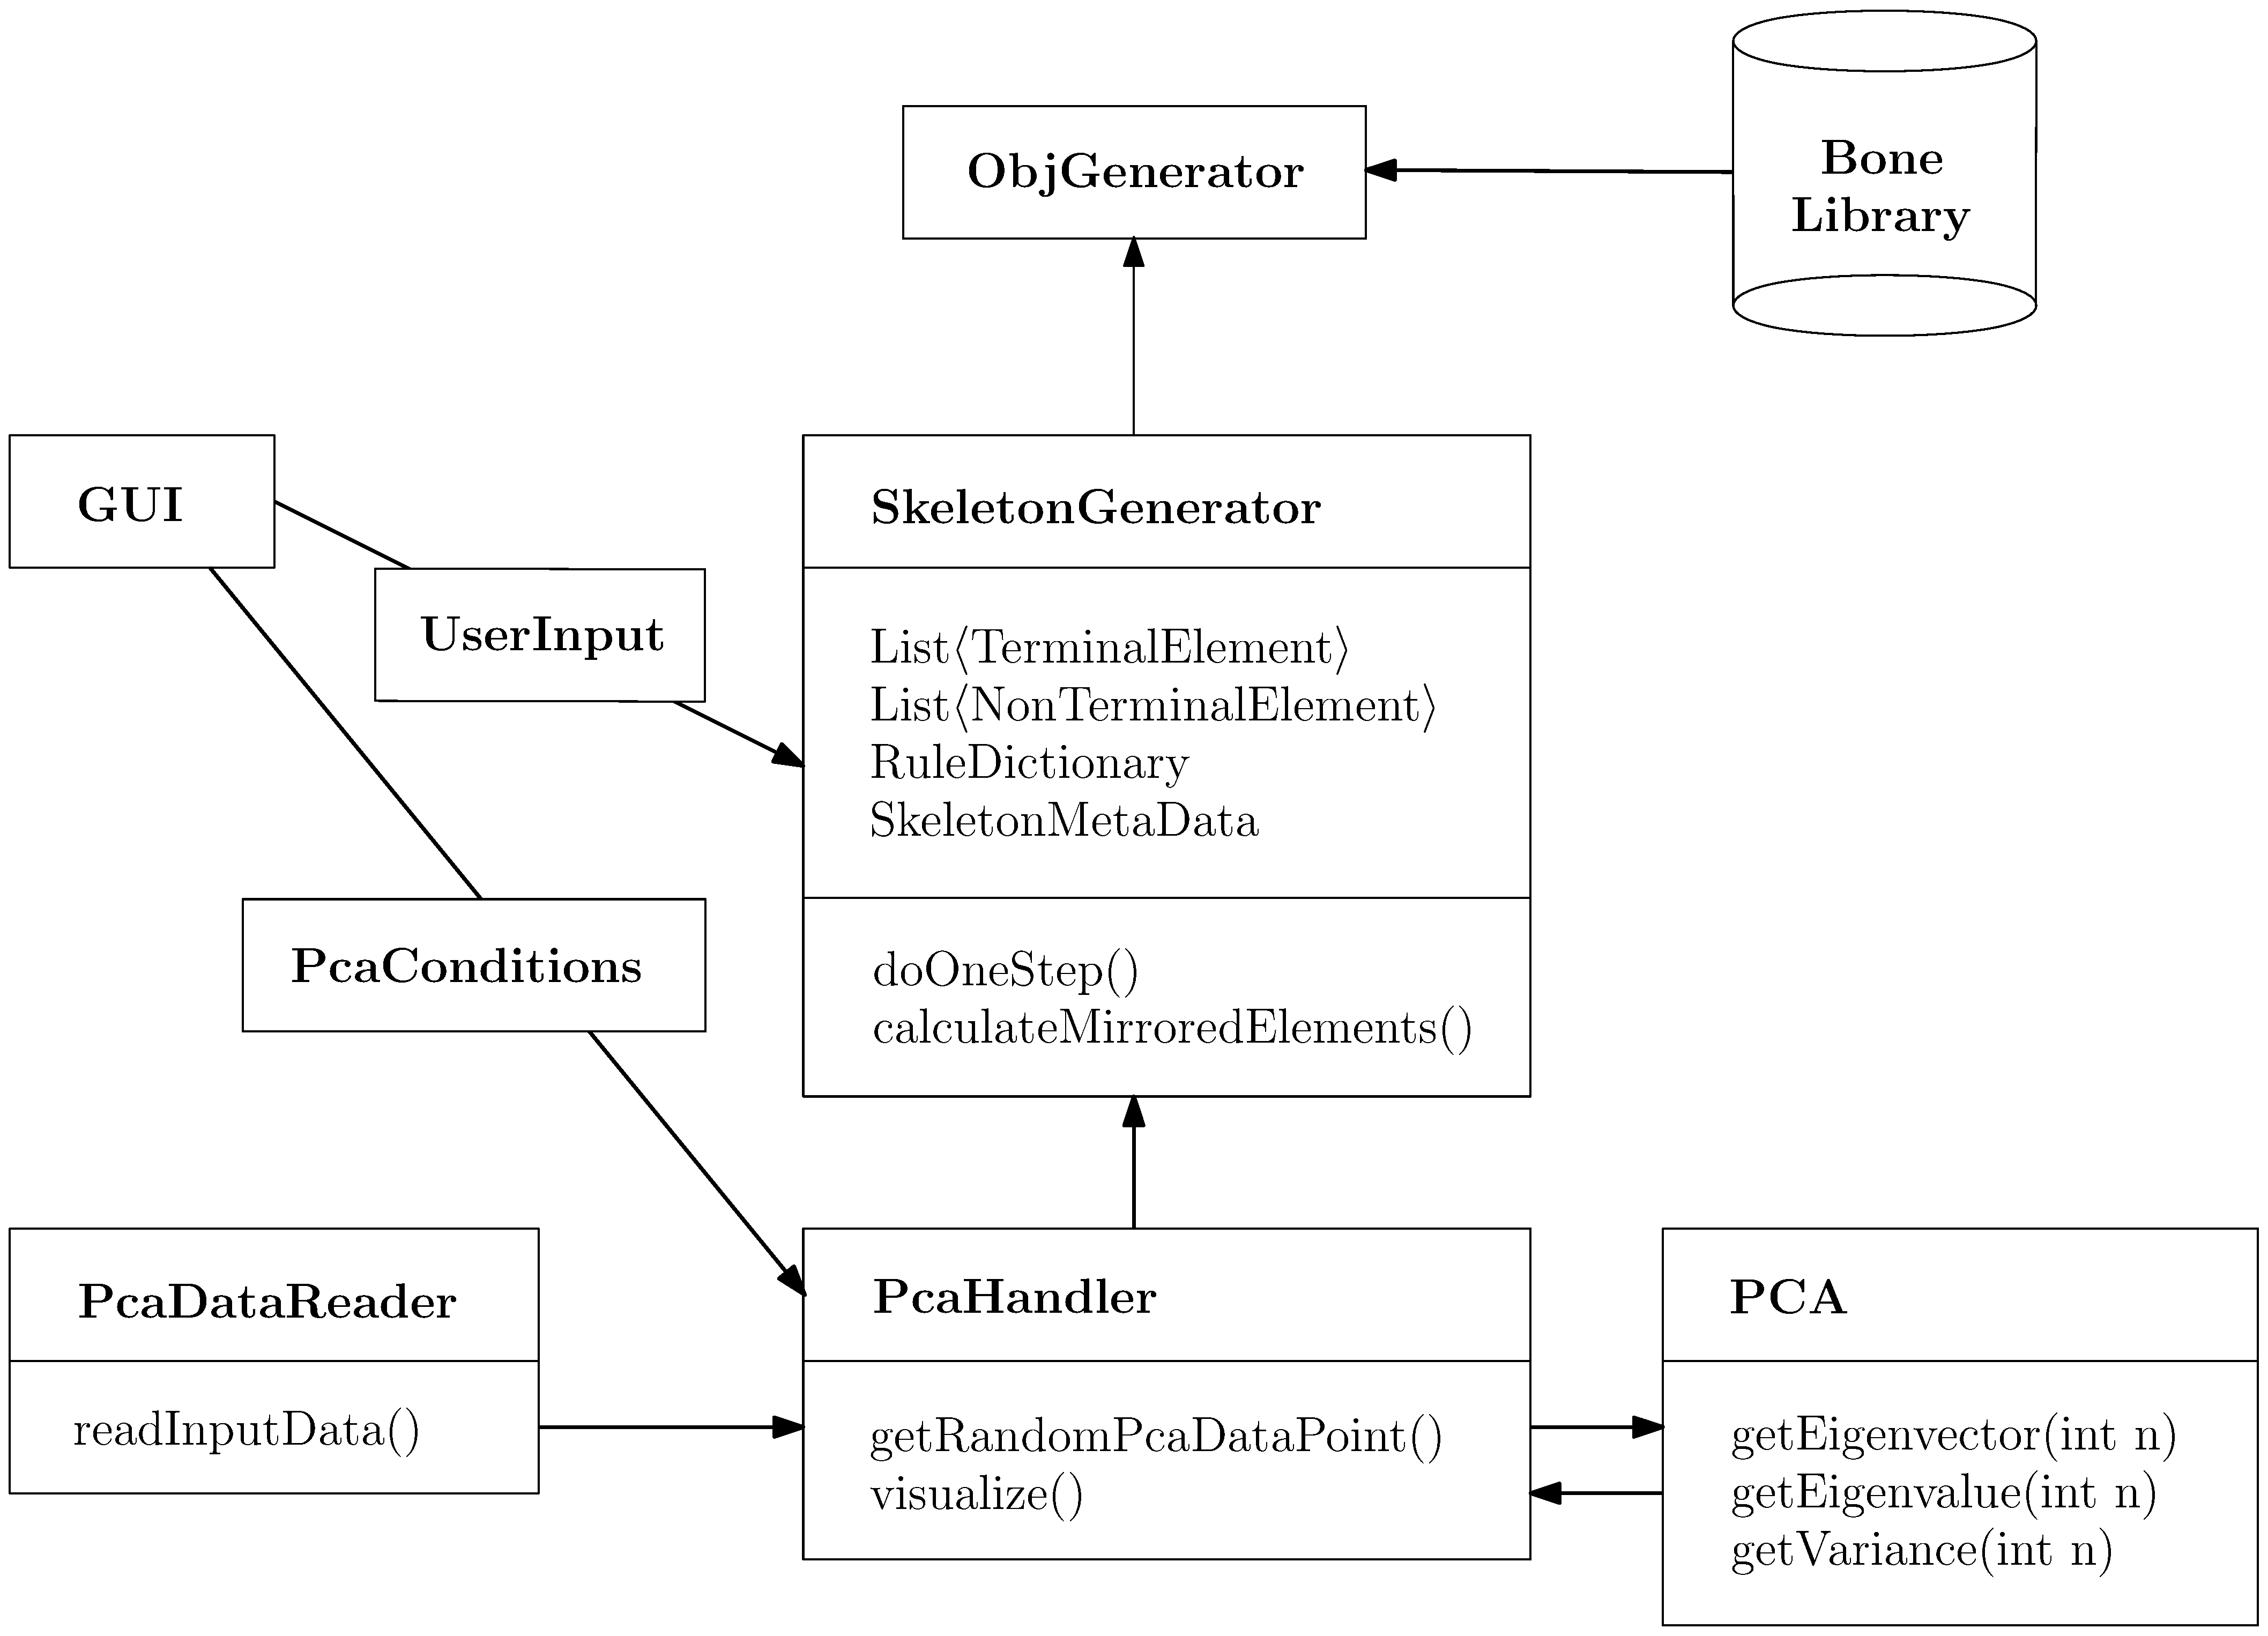
\includegraphics[width=\textwidth]{graphics/classDiagram}
 \caption{Stark vereinfachte Darstellung der Softwarearchitektur. Jeder Kasten steht für eine Klasse, wie in UML-Klassendiagrammen. Pfeile sollen den Datenfluss darstellen.}
 \label{classDiagram}
\end{figure}


%------------------------------------
\section{Dateiformate für 3D-Modelle}

Das einfachste Format zur Darstellung von 3D-Objekten ist das offene Dateiformat Wavefront OBJ \cite{obj}. Es kann nur geometrische Formen speichern, keine zusätzlichen Informationen wie \zb Gelenke und deren Einschränkungen.\\
Andere weit verbreitete Formate sind FBX von Autodesk \cite{fbx} und Alembic \cite{alembic}. Sie bieten mehr Möglichkeiten als OBJ, sind aber auch ungleich aufwändiger programmatisch zu erzeugen.

Um das 3D-Modell des erzeugten Skeletts zu speichern reicht das OBJ-Format aus. Zur Weiterverarbeitung, \zb für Animationen, können die Daten dann leicht in das dann benötigte Dateiformat umgewandelt werden. Für das Laden und Schreiben von OBJ-Dateien wird die Java-Bibliothek Obj \cite{ObjLoader} verwendet.
Sollten in Zukunft zusätzliche Daten exportiert werden können, müsste neu evaluiert werden welches Dateiformat am besten geeignet ist.


% \begin{itemize}
%  \item Jeder Editor geht mit Muskeln und Gelenken anders um. Gibt es ein Dateiformat, das nicht speziell zu einem Editor gehört, dass Bedingungen an die Rotation von Gelenken speichern kann?
%  \item Eigenes Format erzeugen? Dann bräuchte man Plugins um es in verschiedenen Editoren laden zu können. Viel verwendeter Editor: Houdini (kostenlos für Studenten aber nicht Open Source). Oder selbst darstellen (siehe Interaktivität).
% \end{itemize}


%--------------------------------
\section{Transformationsmatrizen}
\label{implementation_detail_matrices}

Jedes Kindelement $k$ im Skelett speichert eine Transformationsmatrix $T_k$, die seine lokalen Koordinaten in das Koordinatensystem des Elternelements $e$ umrechnet (siehe Abschnitt \ref{skeleton_parts} und Abbildung \ref{transformation_matrices_normal}a).
Es treten verschiedene Situationen auf, in denen unterschiedliche Transformationsmatrizen berechnet werden müssen.

In Schritt $4$ des Algorithmus werden \zb alle Elemente, die nicht auf der Wirbelsäule liegen, gespiegelt (siehe Abschnitt \ref{section:overview}). Wird hier einfach eine Spiegelung an der $xy$-Ebene angewendet, so ist das resultierende Koordinatensystem nicht mehr rechtshändig, sondern linkshändig.
Das führt beispielsweise dazu, dass im neuen Koordinatensystem nicht mehr gegen den Uhrzeigersinn, sondern mit dem Uhrzeigersinn gedreht wird. Das kann zu Problemen führen, wenn auf den gespiegelten Elementen Transformationen ausgeführt werden müssen, \va wenn linkshändige und rechtshändige Koordinatensysteme verwendet werden. Außerdem kann es dazu führen, dass die Flächen der 3D-Modelle so interpretiert werden, als würde ihre Vorderseite nach innen zeigen, anstatt nach außen. Wird beim Rendering Backface Culling \cite{backfaceCulling} eingesetzt, führt das dazu, dass diese Flächen nicht sichtbar sind.

Um den Überblick über die Berechnung der Transformationsmatrizen in den verschiedenen Situationen zu behalten, wurden vier Übersichtsgrafiken erstellt (Abbildungen \mbox{\ref{transformation_matrices_normal} a und b}, Abbildung \ref{transformation_matrix_non_mirrored_parent} und Abbildung \ref{transformation_matrix_mirrored_parent}). 
Im Folgenden wird jeweils erklärt welche Situationen sie beschreiben, wann diese auftreten und wie die entsprechenden Transformationsmatrizen berechnet werden.

\begin{itemize}
 \item In Abbildung \ref{transformation_matrices_normal} b ist die Situation dargestellt, die \ua dann auftritt, wenn die Position der Wirbel auf der Wirbelsäule berechnet werden soll. Die Position der Wirbel im globalen Koordinatensystem ist bekannt, ihre Position soll aber im lokalen Koordinatensystem des Elternelements angegeben werden.\\
 Es ist also ein Elternelement $e$ mit zugehörigem Kindelement $k$ gegeben. Für beide Elemente ist die Transformation ins globale Koordinatensystem $T_{eg}$ \bzw $T_{kg}$ bekannt. Die lokale Transformationsmatrix von $k$ ist dann $T_k = T^{-1}_{eg} \cdot T_{kg}$.
 
 \item Die Situation, die entsteht, wenn das Kindelement $k$ eines Elements $e$, das auf der Wirbelsäule liegt, gespiegelt werden soll, ist in Abbildung \ref{transformation_matrix_non_mirrored_parent} dargestellt. Gesucht ist dann die Transformation $T_{k_r}$, die die lokalen Koordinaten des gespiegelten Kindelements $k_r$ in die lokalen Koordinaten von $e$ umwandelt. Das Element $k_l$ entsteht, wenn $k$ einfach an der $xy$-Ebene gespiegelt wird. Dieses Element hat aber kein rechtshändiges Koordinatensystem mehr, sondern ein linkshändiges. Die Grafik macht deutlich, dass $T_{k_r} = T_{eg}^{-1} \cdot T_r \cdot T_{k_lg} \cdot T_{kx}$. Die Matrix $T_r$ spiegelt die $z$-Koordinate und $T_{kx}$ wandelt das linkshändige Koordinatensystem von $k_l$ in das rechtshändige von $k_r$ um. Diese Umwandlung $T_{kx}$ besteht aus einer Verschiebung in $z$-Richtung um die Länge von $k$ in $z$-Richtung und einer Spiegelung an der $xy$-Ebene.
 
 \item Abbildung \ref{transformation_matrix_mirrored_parent} zeigt die Situation, die entsteht, wenn das Elternelement $e$ selbst schon gespiegelt wurde. 
 Es ist also ein gespiegeltes Elternelement $e_r$ gegeben und das dazugehörige gespiegelte Kindelement $k_r$. Gesucht ist die Transformationsmatrix $T_{k_r}$. Wie in Abbildung \ref{transformation_matrix_non_mirrored_parent} sind die linkshändigen Koordinatensysteme der gespiegelten Elemente $e_l$ und $k_l$ gepunktet dargestellt. Die Transformationen $T_{ex}$ und $T_{kx}$ wandeln linkshändige Koordinatensysteme in rechtshändige um. Dann ergibt sich \mbox{$T_{k_r} = T_{ex} \cdot T_k \cdot T_{kx}$}, da $T_k = T_{k_l}$.
\end{itemize}

\begin{figure}
 \centering
 \subfloat[Transformation ins globale Koordinatensystem]{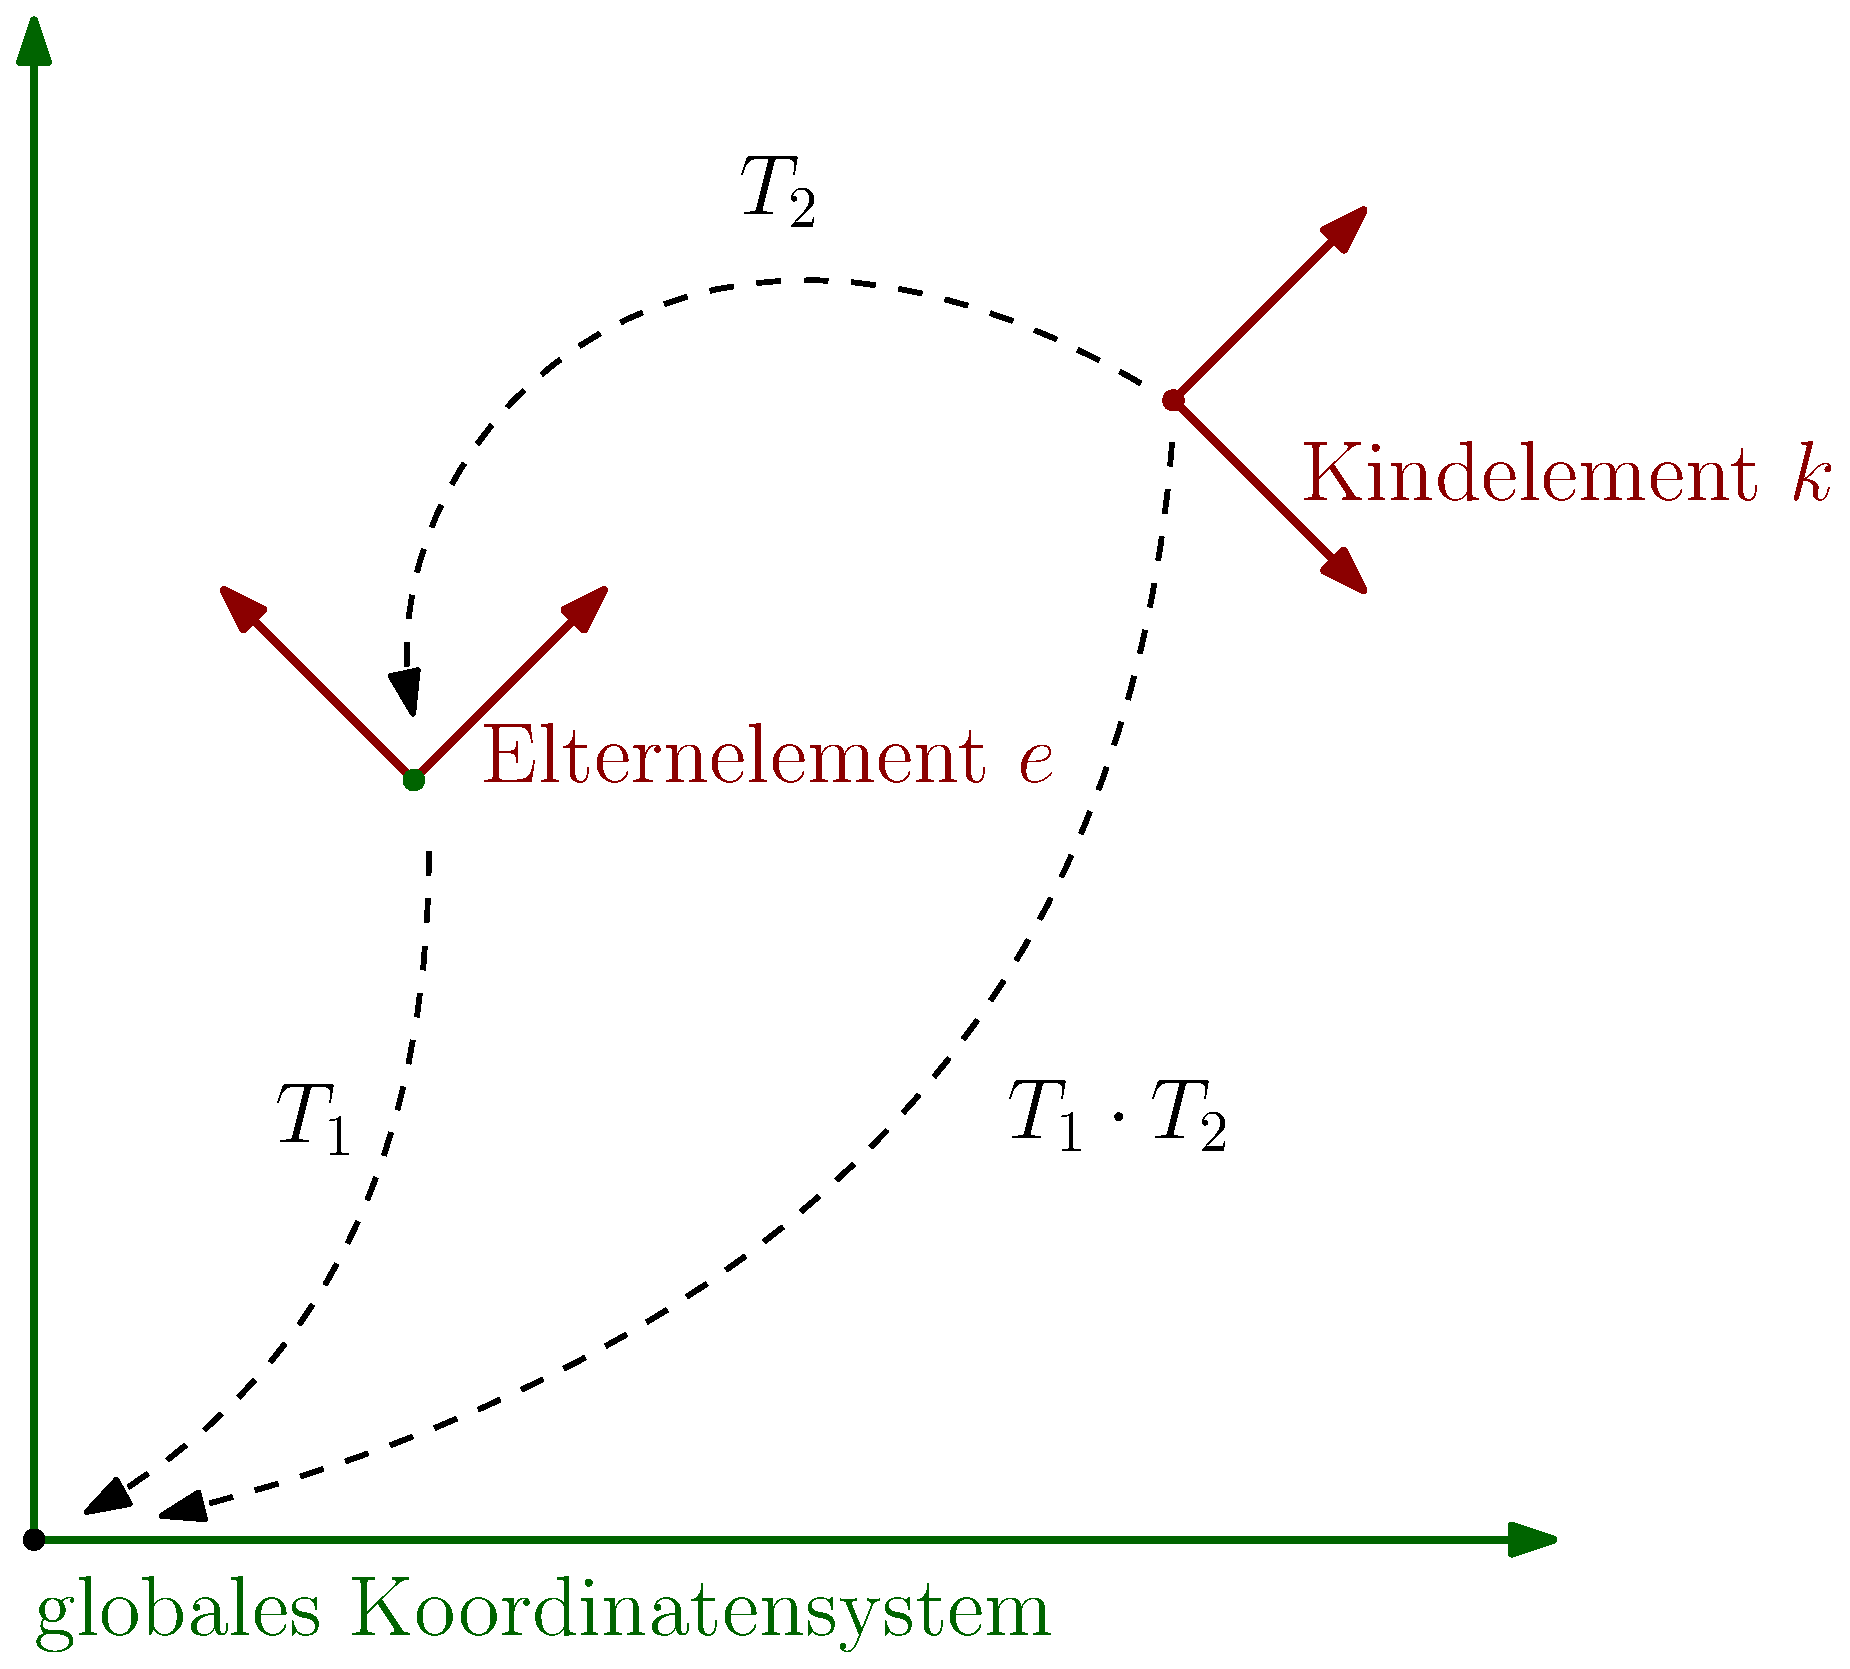
\includegraphics[width=0.5\textwidth]{graphics/transformation_matrices}}~
 \subfloat[vorgegebene globale Position]
 {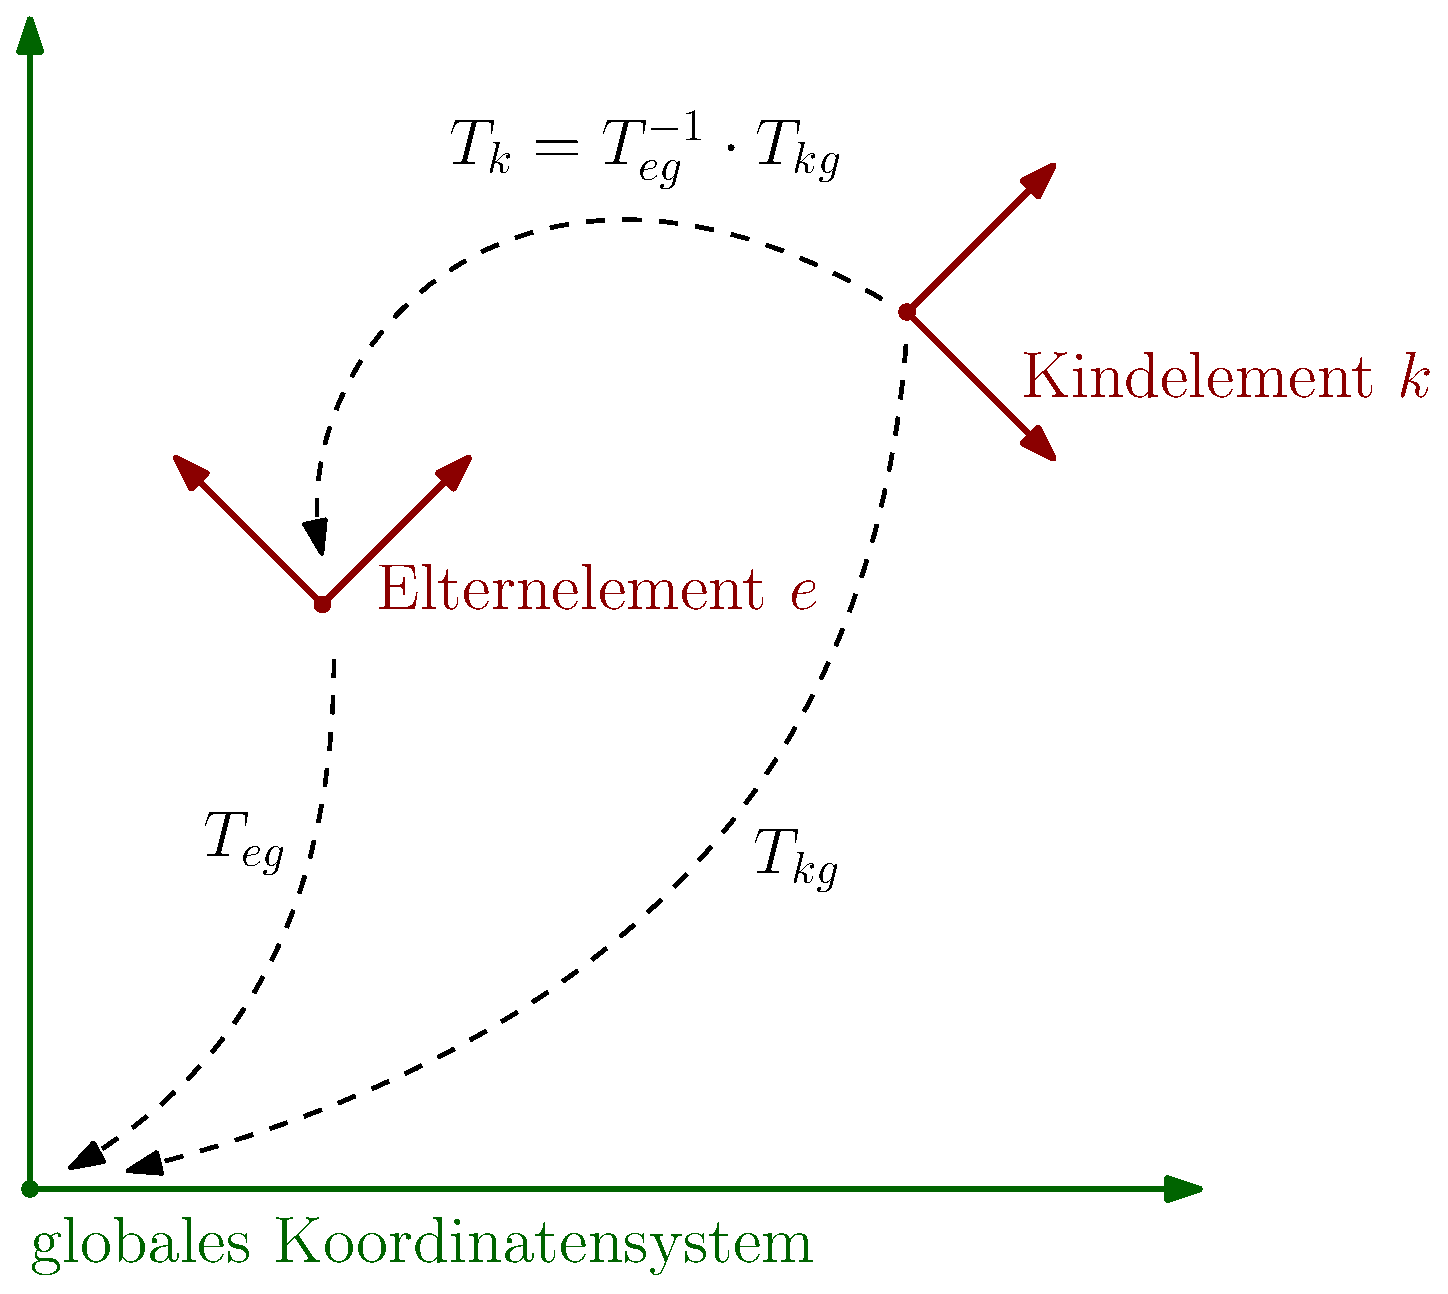
\includegraphics[width=0.5\textwidth]{graphics/transformation_matrices_spine}}
 
 \caption{Jedes Kindelement $k$ speichert eine Transformation $T_k$ ins lokale Koordinatensystem seines Elternelements $e$. (a) Ist $T_k$ gegeben, so lässt sich die Transformation $T_{kg}$ des lokalen Koordinatensystems von $k$ ins globale Koordinatensystem durch $T_{kg} = T_{eg} \cdot T_k$ berechnen. (b) Ist $T_{kg}$ gegeben, so lässt sich $T_k = T^{-1}_{eg} \cdot T_{kg}$ berechnen.} 
 \label{transformation_matrices_normal}
\end{figure}

\begin{figure}
 \centering
 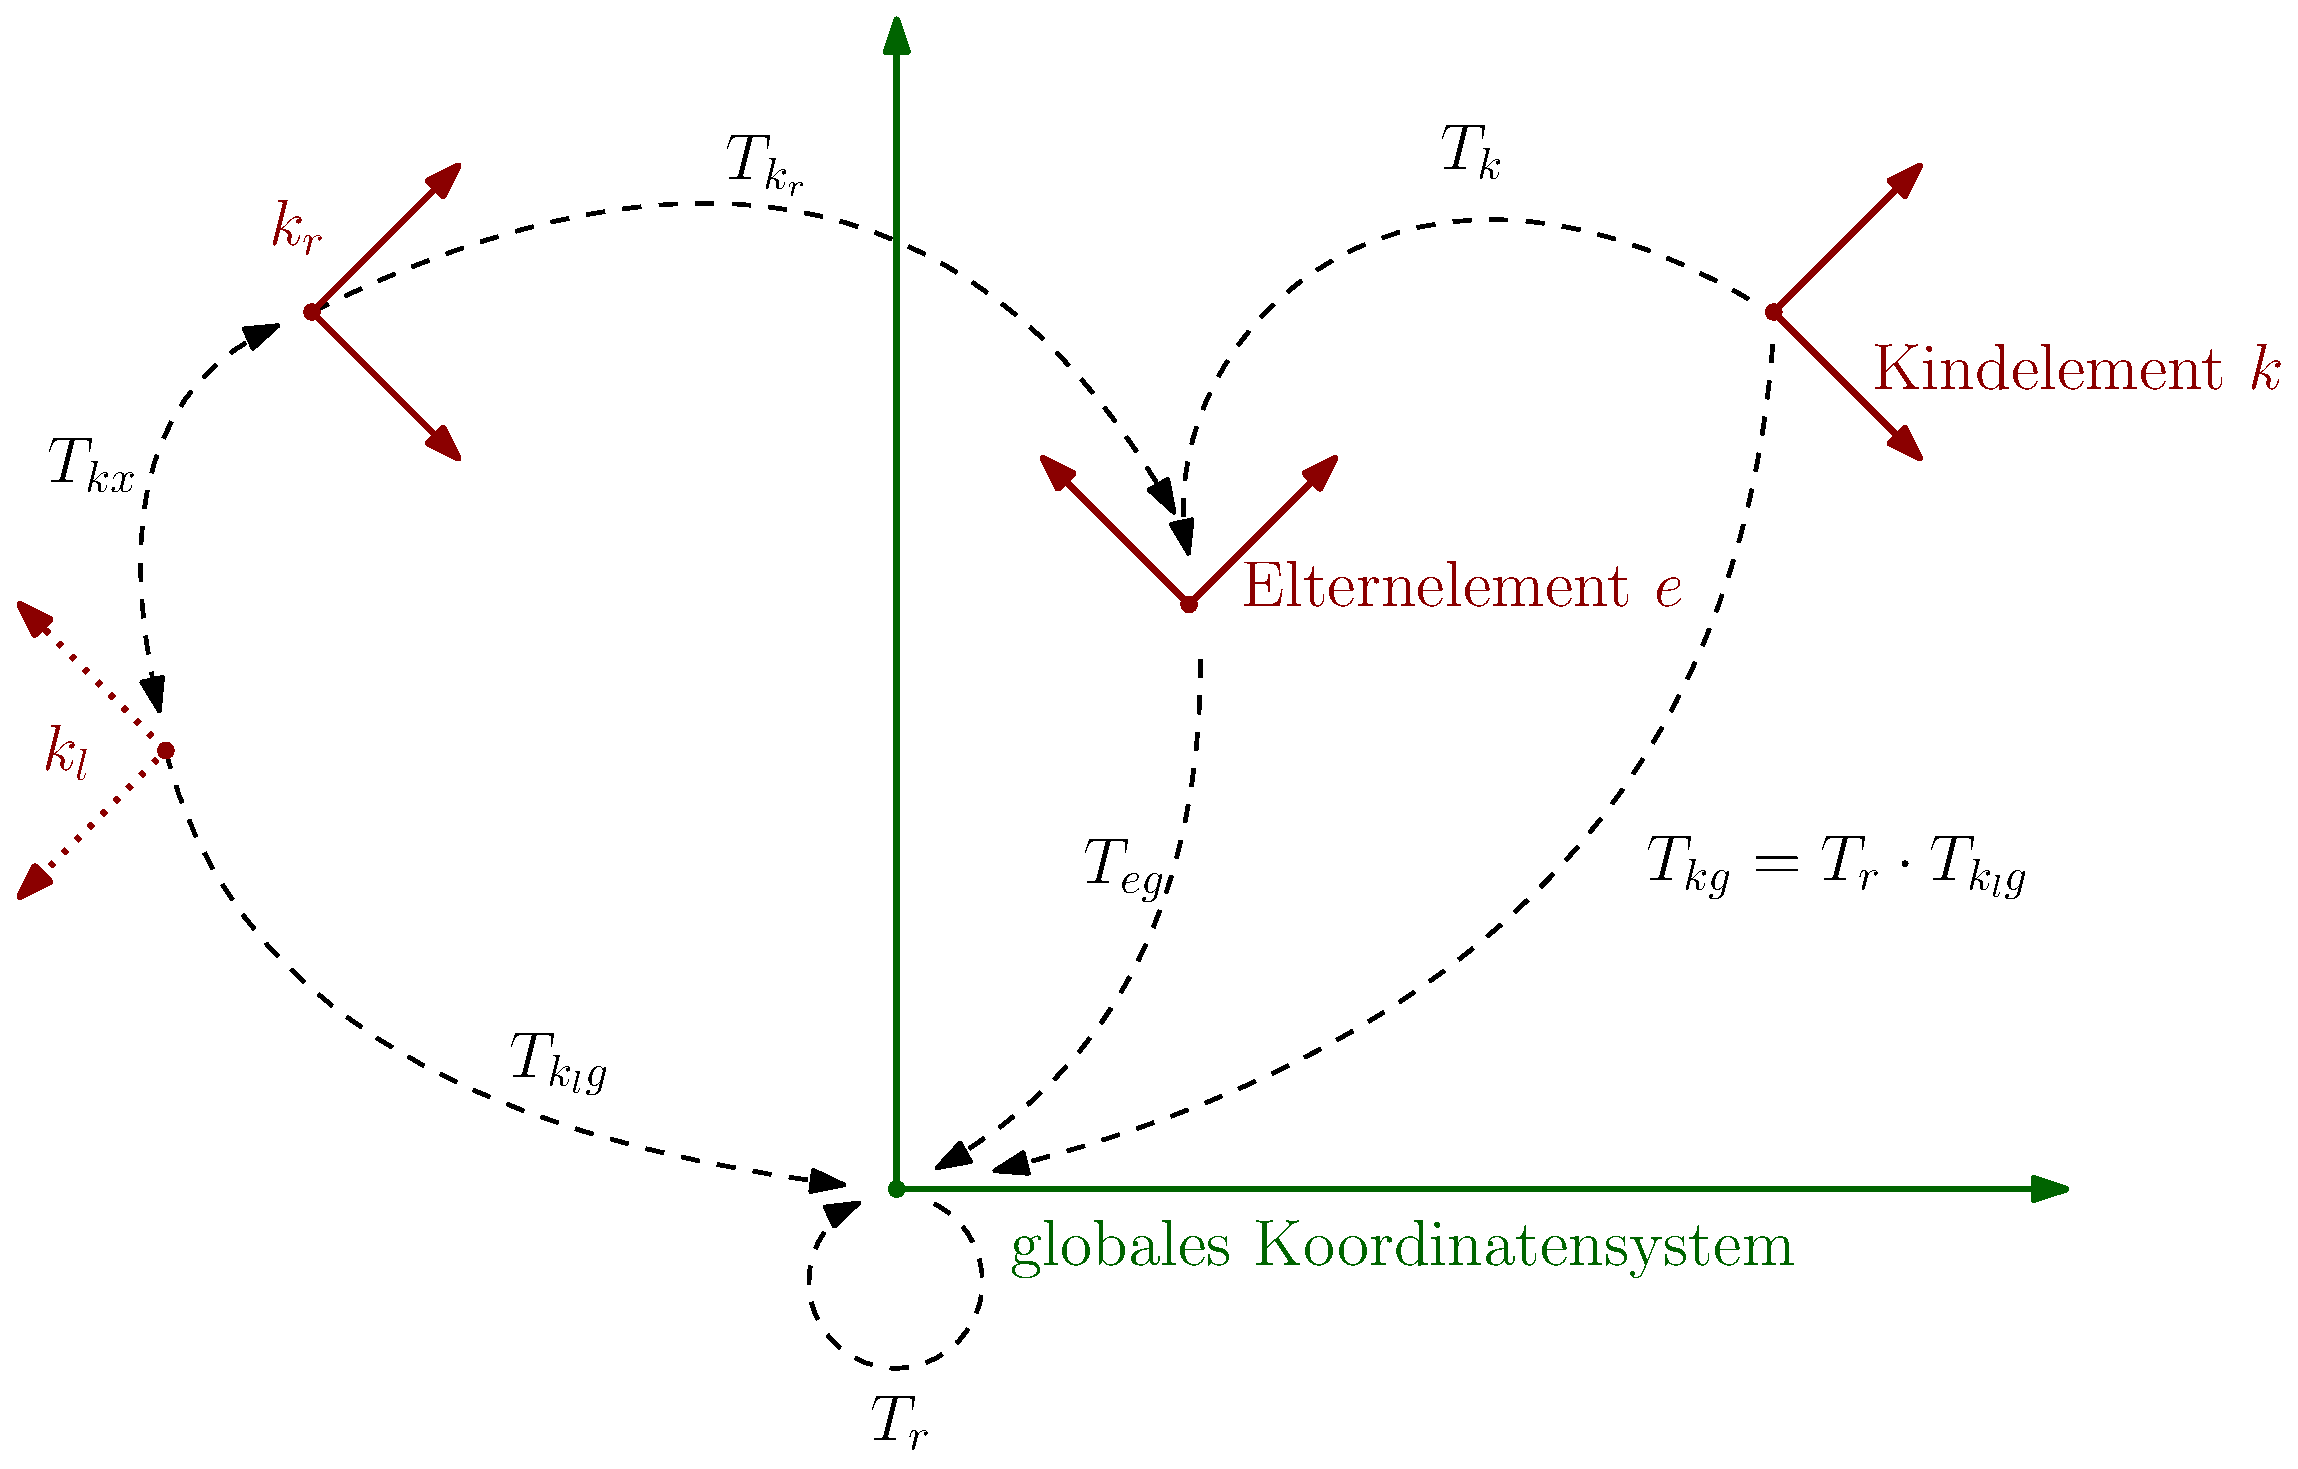
\includegraphics[width=0.9\textwidth]{graphics/transformation_matrices_non_mirrored_parent}
 \caption{Die Transformationsmatrix $T_{k_r}$ des gespiegelten Kindelements $k_r$ lässt sich berechnen durch $T_{k_r} = T_{eg}^{-1} \cdot T_r \cdot T_{k_lg} \cdot T_{kx}$. Die Matrix $T_r$ spiegelt die $z$-Koordinate und $T_{kx}$ wandelt das linkshändige Koordinatensystem von $k_l$ in das rechtshändige von $k_r$ um.}
 \label{transformation_matrix_non_mirrored_parent}
\end{figure}

\begin{figure}
 \centering
 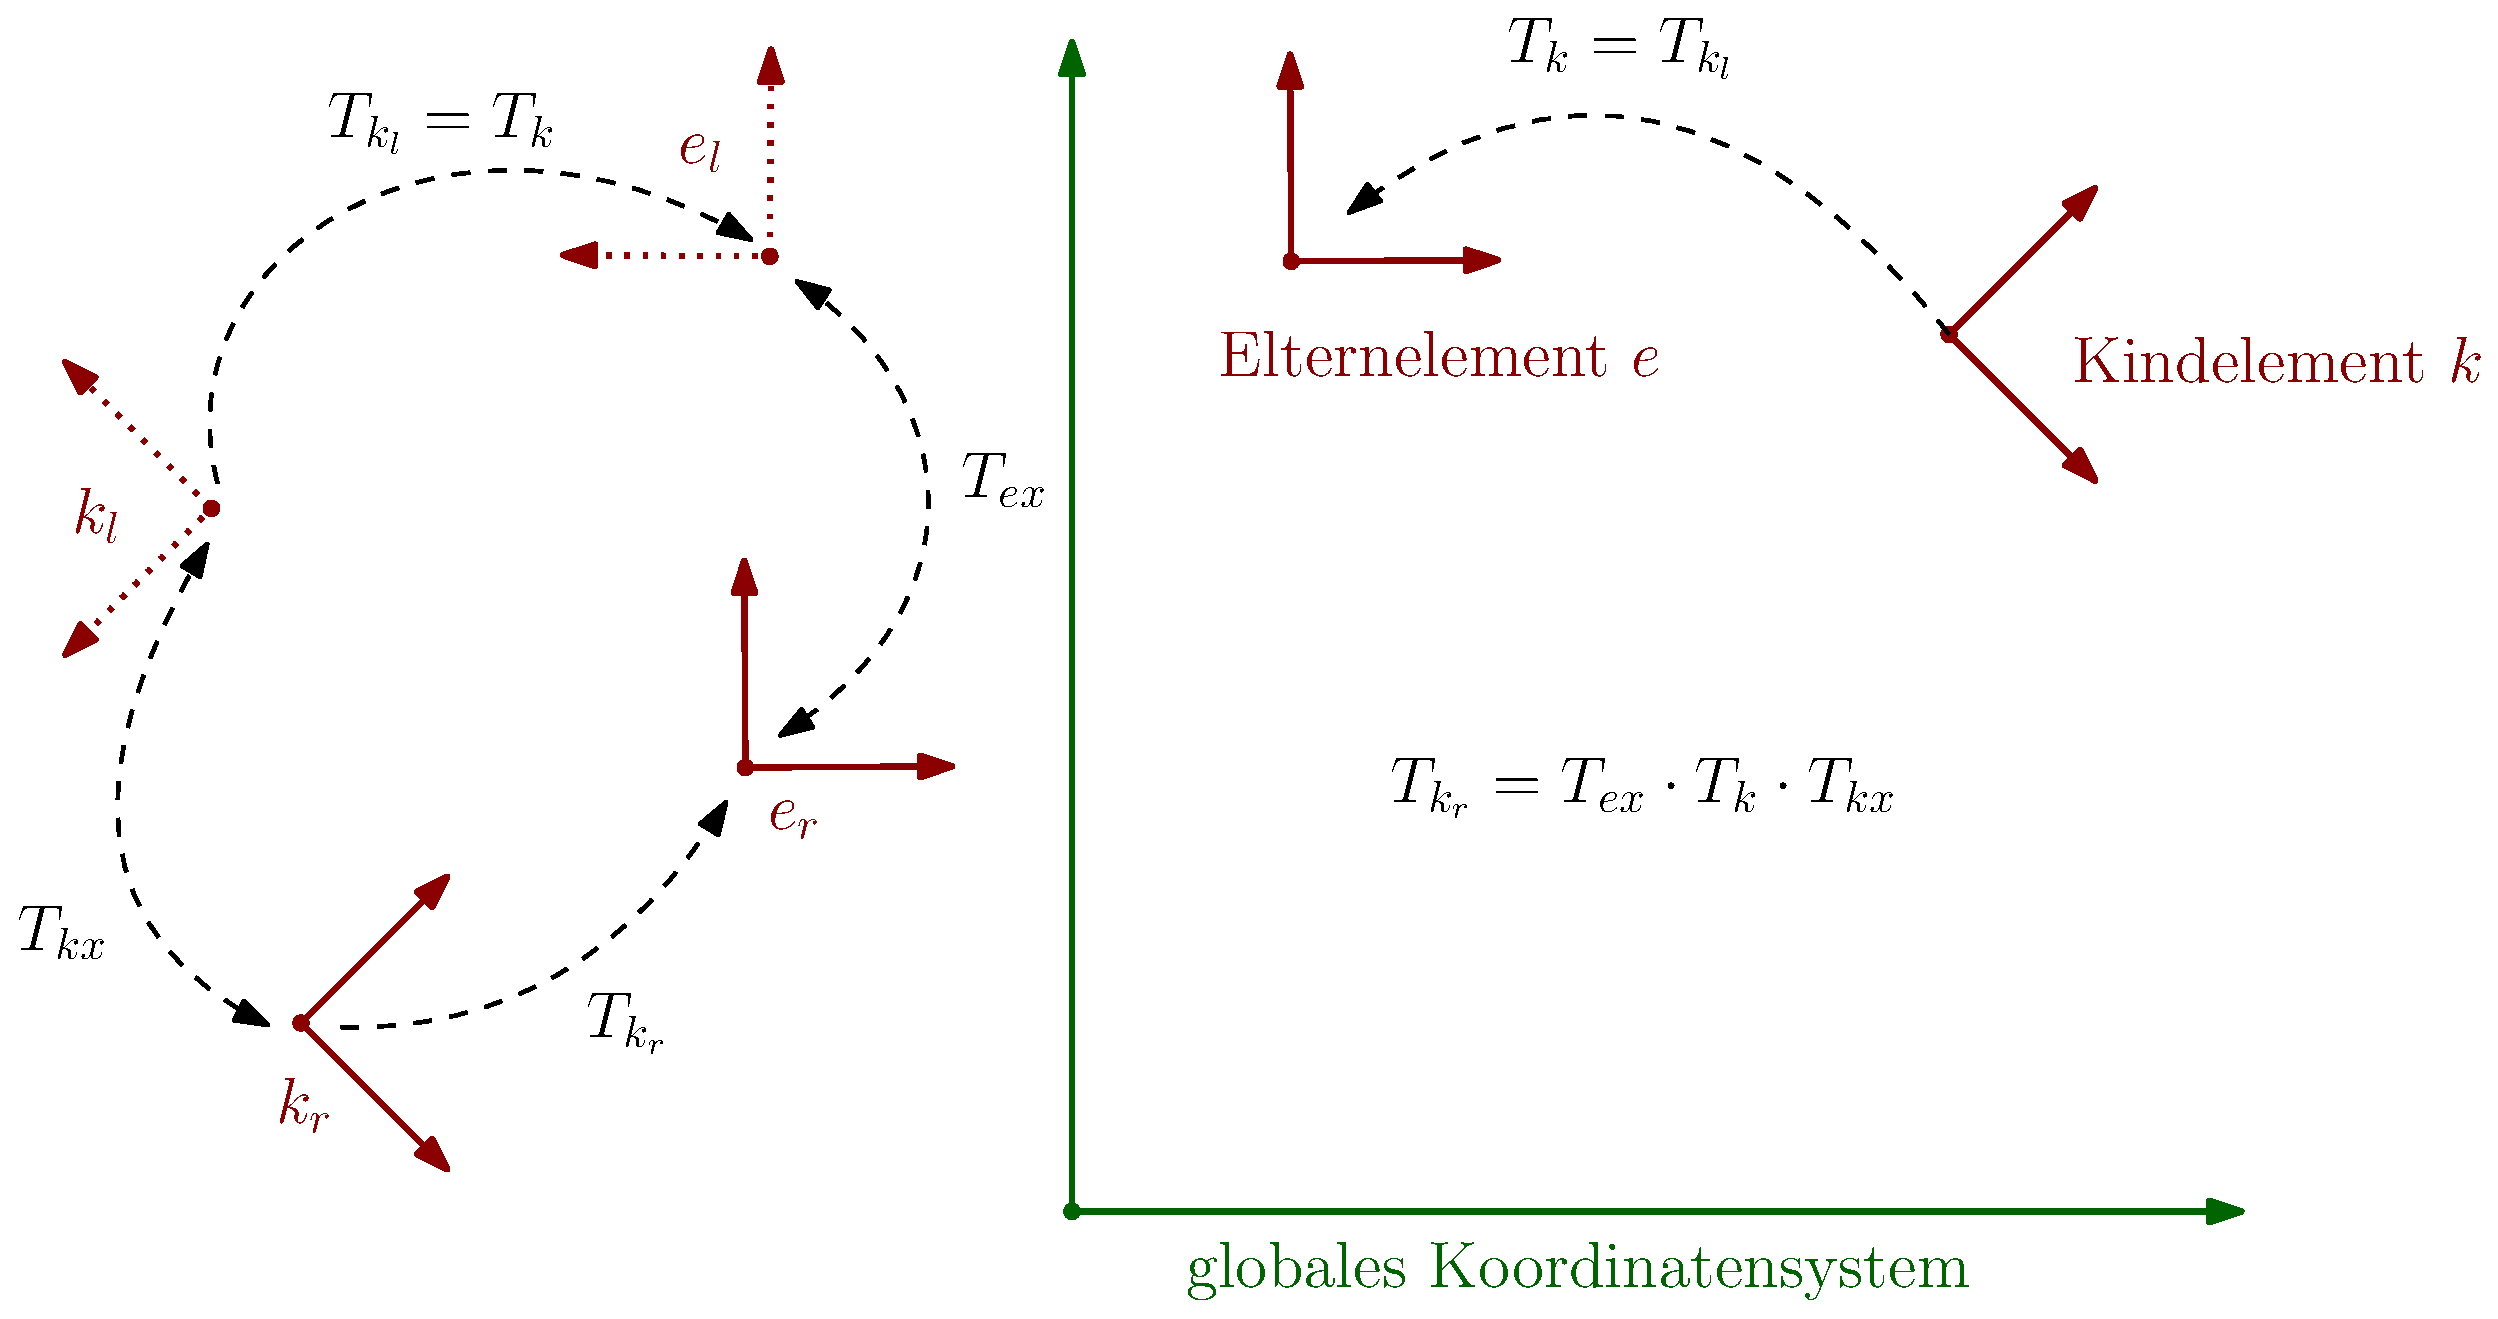
\includegraphics[width=0.9\textwidth]{graphics/transformation_matrices_mirrored_parent}
 \caption{Die Transformationsmatrix $T_{k_r}$ des gespiegelten Kindelements $k_r$ eines ebenfalls gespiegelten Elternelements $e_r$ lässt sich berechnen durch $T_{k_r} = T_{ex} \cdot T_k \cdot T_{kx}$. Die Matrizen $T_{ex}$ und $T_{kx}$ wandeln das linkshändige Koordinatensystem von $e_l$ \bzw $k_l$ in das rechtshändige von $e_r$ \bzw $k_r$ um.}
 \label{transformation_matrix_mirrored_parent}
\end{figure}


%------------
\section{PCA}
\label{implementation_detail_pca}

%- - - - - - - - - - - - - - - - -
\subsection{Annotation der Bilder}

Die Bilder der Skelette wurden folgendermaßen für die Datenerhebung vorbereitet:
 
 \begin{enumerate}
  \item Zuschneiden des Bildes, so dass möglichst nur das Skelett mit wenig Rand außen herum zu sehen ist.
  \item Einfügen in eine $1000 \times 1000$ Pixel große Bildumgebung.
  \item Vergrößern des Bildes, sodass es möglichst viel Platz innerhalb der Bildumgebung einnimmt, ohne die Seitenverhältnisse zu verändern.
  \item Verschieben innerhalb der Bildumgebung an den unteren Rand und horizontal in die Mitte.
 \end{enumerate}

 Ist das geschehen kann die Lage der Wirbelsäule und die Länge der Knochen der Extremitäten annotiert werden.
 
Die Annotation der Bilder wurde per Hand mit dem Programm Inkscape \cite{inkscape} durchgeführt. Es kann verwendet werden um Vektorgrafiken zu erstellen und zu bearbeiten.\\
Für jedes zu markierende Element wurde eine Strecke oder eine Bézierkurve eingefügt und mit einem vorher festgelegten Namen benannt. Diese Elemente wurden dann durch Inkscape als Pfade in der erzeugten svg-Datei gespeichert. Aus dieser Datei wurden dann automatisiert die eingetragenen Pfade mit ihren Koordinaten ausgelesen.

Folgende Details sind wichtig zu beachten, damit dieser Vorgang reibungslos abläuft. 
\begin{itemize}
 \item Man kann in Inkscape einstellen, dass Koordinaten immer absolut angegeben werden. Das ist sinnvoll um die Koordinaten leichter auslesen zu können.
 \item Der Ursprung des Koordinatensystems in Inkscape ist unten links, im svg-Format ist er aber oben links.
 \item Ebenen in Inkscape sollten nicht verschoben sein, sonst verschieben sich mit ihnen auch die Koordinaten.  
\end{itemize}

%- - - - - - - - - - - - - - - - - - - - - - - - -
\subsection{Anpassung des Verlaufs der Wirbelsäule}
\label{smooth_spine}

Die Wirbelsäule, die durch einen Punkt im PCA-Raum vorgegeben wird, besteht aus drei einzelnen Bézierkurven. Diese Bézierkurven haben an den Punkten, an denen sie zusammenstoßen die gleichen Koordinaten. Die Gesamtkurve der Wirbelsäule muss an diesen Punkten aber nicht unbedingt differenzierbar sein.
Deshalb müssen vor der Weiterverwendung die jeweils nächsten Kontrollpunkte vor und nach dem Kontaktpunkt verschoben werden. \\
Das wurde hier so gemacht, dass die zu verschiebenden Kontrollpunkte jeweils um den gleichen Winkel aber in gegensätzliche Richtungen rotiert wurden (siehe Abbildung \ref{smooth_spine}). 

Grundsätzlich könnten die Kontrollpunkte beliebig auf einer gewählten Tangente des Kontaktpunkts platziert werden (rot im Bild) um eine übereinstimmende Steigung zu bekommen. Um den Verlauf der Wirbelsäulenteile möglichst wenig zu verändern ist es von Vorteil auch die Kontrollpunkte möglichst wenig zu verschieben. Man könnte die Punkte \zb auch senkrecht auf die Tangente projizieren. Welches Verfahren angewendet wird, ist jedoch nicht von großer Bedeutung. 

\begin{figure}
 \subfloat[vorher]{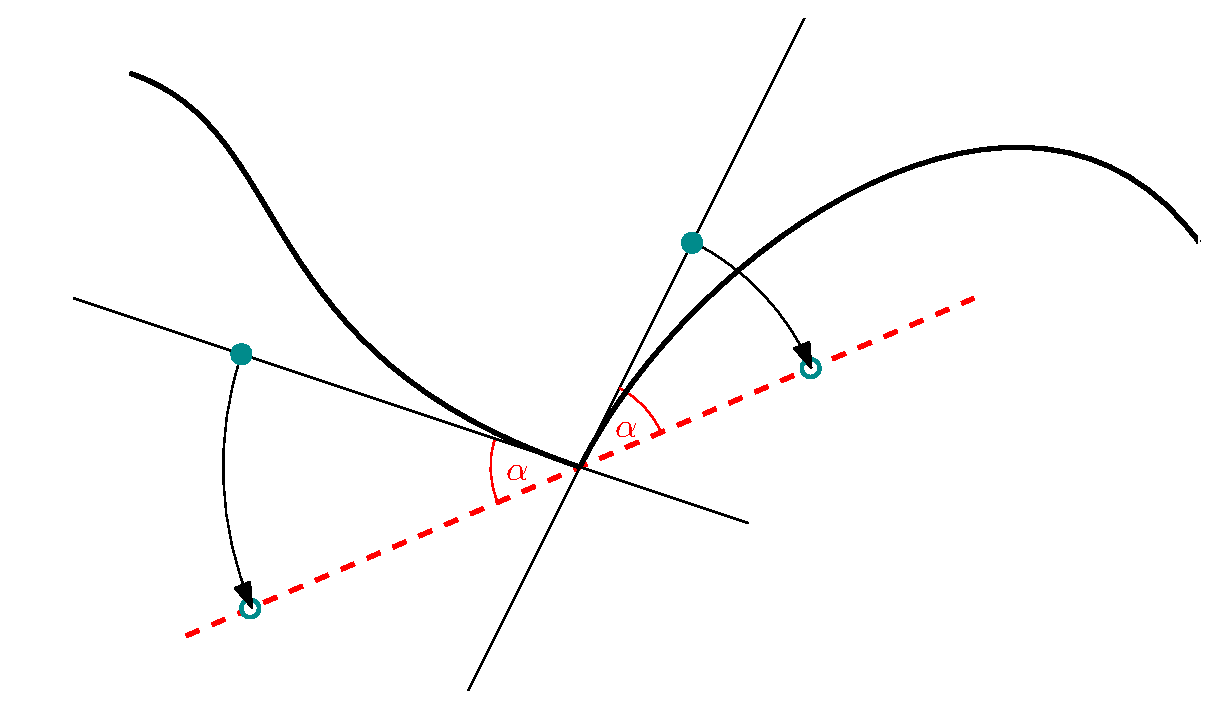
\includegraphics[width=0.5\textwidth]{graphics/smooth_spine1.eps}}
 \qquad
 \subfloat[nachher]{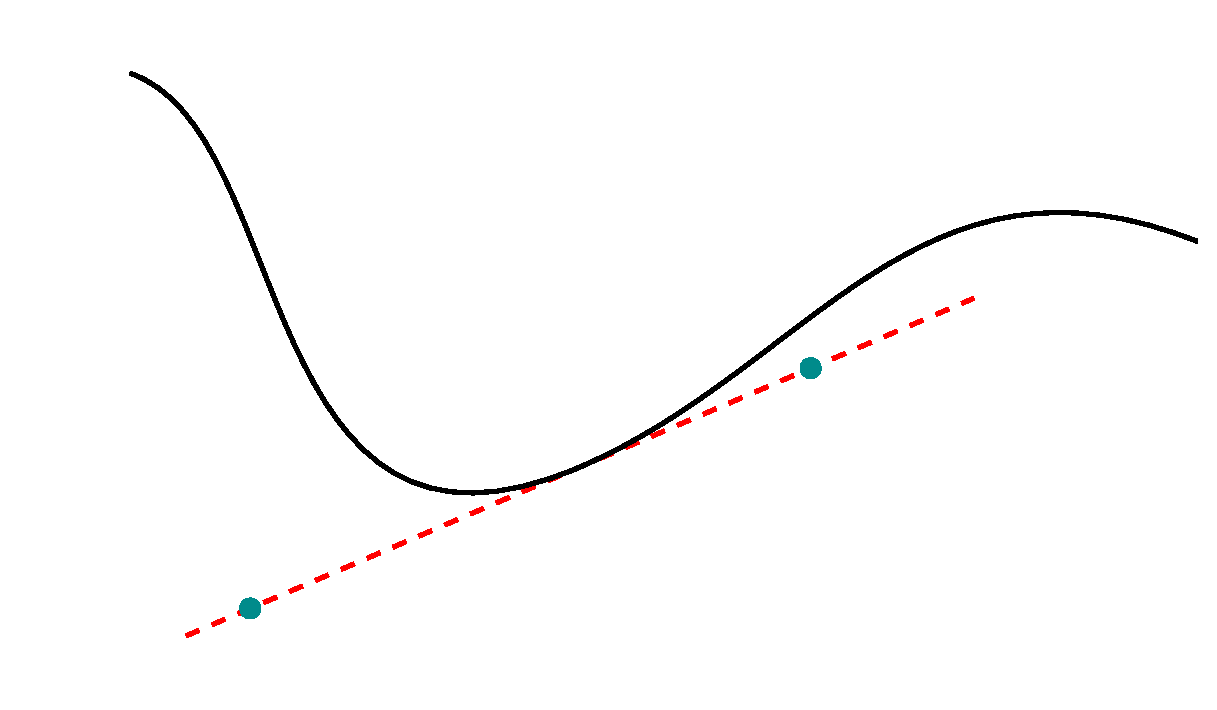
\includegraphics[width=0.5\textwidth]{graphics/smooth_spine2.eps}}
 \caption{Anpassung der Kontrollpunkte der Wirbelsäulenteile, wenn die Steigung an den Kontaktpunkten ungleich ist. Die beiden Teile der Wirbelsäule und die Steigung am Kontaktpunkt sind hier in schwarz dargestellt. Die zu drehenden Kontrollpunkte in cyan. In rot ist die resultierende Steigung und der Winkel, der für die Drehung verwendet wird, zu sehen.}
 \label{smooth_spine}
\end{figure}


%------------------------------------------------------
\section{Probleme der Positionierung von kurzen Beinen}
\label{leg_positioning_short_legs}

Wie in Absatz \ref{leg_algo} bereits beschrieben, treten bei der Ausrichtung sehr kurzer Beine ein paar Probleme auf. Diese werden im Folgenden kurz umrissen. Da die Beine in diesen Fällen aber sehr kurz sind, hat die konkrete Positionierung in diesen Fällen keine große Auswirkung auf die Gesamtwirkung des Skeletts. 

\begin{enumerate}
 \item % Bodenhöhe nicht von Gelenk aus gemessen
   Bei der Berechnung der Bodenhöhe wird die Beinlänge von den entsprechenden Kontrollpunkten der Bézierkurve aus gemessen, da die Position des Schulterblatts \bzw des Beckenknochens in diesem Stadium noch nicht klar ist. Deshalb kann es bei sehr kurzen Beinen sein, dass der Abstand zwischen Boden und Gelenk länger als das Bein ist und der Boden nicht erreicht werden kann.
   
   In diesem Fall wird das Bein einfach komplett ausgestreckt, senkrecht nach unten positioniert. Da der Abstand zwischen dem Hüft- \bzw Schultergelenk und dem Kontrollpunkt der Bézierkurve nicht sehr groß ist, fällt auch der Abstand zur Bodenhöhe nicht allzu sehr auf.
   
 \item % keine starke Änderung durch Drehung der Gelenke
   Bei sehr kurzen Knochen ändert sich der Abstand zum Boden durch Drehung der Gelenke nicht so stark wie bei langen Knochen. Wenn der Winkel sich zu wenig ändert, wird aber davon ausgegangen, dass die Winkeländerung zu klein ist und alle Änderungen sofort wieder zurückgesetzt wurden. Deshalb wird die Winkeländerung dann für die nächste Iteration stärker verkleinert. Das ist aber in diesem Fall kontraproduktiv. Der Algorithmus schafft es dann nämlich nicht mehr die Knochen in die richtige Lage zu bringen, da der Bewegungsspielraum dadurch zu stark eingeschränkt wird.
   
   Dem könnte man entgegenwirken, indem man abfragt wie oft die Drehungen in der jeweiligen Iteration zurückgesetzt wurden, anstatt die Änderung des Abstandes zum Boden zu messen.
   
 \item % ganz kurze Beine
   Bei wirklich sehr kurzen Beinen (hier eine Gesamtlänge unter 5) macht es gar keinen Sinn sie anzuordnen, da man sie kaum sieht. Außerdem tritt hier der Effekt auf, der in Punkt 2 schon beschrieben wurde.
   
 \item % Beinstartpos unter Bodenhöhe
   Die Knochen der Beine können schon vor der ersten Iteration unterhalb der Bodenhöhe liegen. Das tritt auf, wenn mindestens ein Paar Beine sehr kurz ist und die Wirbelsäule an den Ansatzpunkten auf sehr unterschiedlicher Höhe liegt (siehe auch Absatz \ref{floor_height} zur Berechnung der Bodenhöhe).
   %\todo{Beispiel: Dimetrodon}
   
   In diesem Fall ist der Algorithmus natürlich nicht anwendbar. Das Bein wird dann einfach senkrecht nach unten ausgerichtet und mit einem Fuß versehen, der mit der Sohle auf dem Boden steht.
   
 \item % Gelenkoffsets
   Bei kurzen Beinknochen kann es dazu kommen, dass der Oberschenkel nicht näher zum Boden bewegt werden kann, weil er schon aufliegt, aber Schienbein und Hand durch das Gelenkoffset (siehe Abschnitt \ref{bone_models} zur Positionierung der Knochenmodelle) über dem Boden schweben und nicht näher zum Boden bewegt werden können.
   %\todo{Beispiel Krokodil (siehe auch Screenshot)}
\end{enumerate}







